\documentclass[11pt]{article}

\usepackage[margin=1in]{geometry}
\usepackage{amsmath,amssymb,amsthm}
\usepackage{graphicx}
\usepackage{booktabs}
\usepackage{multirow}
\usepackage{xcolor}
\usepackage[numbers,sort&compress]{natbib}
\usepackage[colorlinks=true,linkcolor=black,citecolor=blue,urlcolor=blue]{hyperref}

\graphicspath{{figures/}}
\setlength{\emergencystretch}{2em}
\newcommand{\sr}{\mathrm{SR}}
\newcommand{\mdd}{\mathrm{MDD}}

\title{\bfseries Do Bootstrap Confidence Intervals for Backtest Statistics
Cover?\\ A Controlled Study Under Serial Dependence}

\author{Eugen Soloviov\thanks{Independent Researcher. ORCID:
\href{https://orcid.org/0009-0006-3148-111X}{0009-0006-3148-111X}.
Correspondence: \href{mailto:suenot@gmail.com}{suenot@gmail.com}.
Code to reproduce every number and figure:
\url{https://github.com/suenot/bootstrap-coverage}.}}

\date{}

\begin{document}
\maketitle

\begin{abstract}
Practitioners are widely advised to attach uncertainty to a backtest by
resampling its daily returns or its trades with replacement and reading
confidence intervals off the bootstrap distribution. We give this advice a
controlled coverage test. Five return-generating processes with
\emph{exactly} known annualized Sharpe ratios---iid Gaussian, iid Student-$t$,
AR(1), GARCH(1,1), and Markov regime-switching volatility---are simulated at
$T\in\{250,1000,4000\}$ days, and fourteen interval methods (Lo's iid and
HAC-adjusted standard errors; iid percentile, basic, and BCa bootstraps;
trade-level resampling with fixed and threshold-crossing episodes; stationary
and circular block bootstraps with swept and automatically selected block
lengths) are scored on $6{,}000$ experiments at $90\%$ and $95\%$ nominal. The
verdict splits four ways. Where returns are truly iid the advice is sound:
pooled over $2{,}400$ iid experiments the percentile bootstrap covers $0.954$
$[0.945,0.961]$ at $95\%$ nominal, heavy tails down to $\nu=5$ included.
Under autocorrelation it breaks, and not as a small-sample effect: at
AR(1) $\phi=0.3$ the per-bar iid bootstrap covers $0.841$ at $95\%$
nominal---a nominal $5\%$ miss rate that is really $16\%$---converges with
sample size to a non-nominal limit ($0.812\to0.854$ from $T=250$ to $4000$,
against an analytic asymptote of $0.850$), and is not rescued by the BCa
construction ($0.838$): the failure is the resampling scheme, not the interval
formula. Resampling whole multi-day \emph{trades} turns out to be an
accidental non-overlapping block bootstrap and is calibrated at the same
$\phi=0.3$ ($0.946$) so long as the trade unit exceeds the dependence length;
volatility dynamics alone (GARCH, regimes) barely hurt Sharpe coverage. For
maximum drawdown the news is uniformly bad: the bootstrap ``$5\%$ worst-case''
drawdown quantile is optimistic everywhere---its realized exceedance
probability is $0.08$--$0.10$ even on iid Gaussian returns, $0.13$--$0.17$
under regime volatility, and $0.23$ under AR(1) at both path lengths; block
methods repair only the autocorrelation channel. Practical recipe: never
resample dependent PnL per bar; default to an automatic-block-length block
bootstrap or Lo's HAC standard error; treat bootstrap drawdown quantiles as
lower bounds.
\end{abstract}

\section{Introduction}

A backtest produces a point estimate---an annualized Sharpe ratio, a maximum
drawdown---and a point estimate invites a confidence interval. The advice
circulating in practitioner writing is appealingly simple: resample the
backtest's daily returns, or its individual trades, with replacement; recompute
the statistic on each resample; and read the interval off the quantiles of the
bootstrap distribution \citep{aronson2006evidence}.\footnote{The specific
trade-level resampling recipe we test, including the choice of the trade as the
resampling unit, follows the author's own earlier practitioner writing (a
market-making blog post on Monte Carlo analysis of backtests). This paper is a
controlled self-audit of advice the author has himself circulated, not an
attack on a third party.} The procedure inherits the prestige of the bootstrap
\citep{efron1979bootstrap} while quietly discarding its central assumption:
resampling individual observations is justified for independent data, and
strategy PnL streams are not independent. Overlapping positions induce
autocorrelation; volatility clusters \citep{bollerslev1986generalized} and
switches regimes \citep{hamilton1989new}. A bootstrap that destroys this
dependence understates the sampling variability of mean-like statistics under
positive dependence, and the intervals it produces may cover the truth far less
often than advertised.

How much less often, for the statistics practitioners actually report? The
question is empirical and, to our knowledge, unanswered. The block-bootstrap
literature (Section~\ref{sec:related}) proved decades ago that dependence
requires resampling blocks, and \citet{ledoit2008robust} showed that classical
\emph{two-sample} Sharpe tests over-reject under dependence; but the one-sample
\emph{coverage} of the intervals attached to a single backtest's Sharpe ratio
and maximum drawdown---across the iid, trade-level, block, and analytic methods
a practitioner might pick---has not been measured under a known truth.

We measure it. Five families of daily-return processes are constructed so that
the population annualized Sharpe ratio is known \emph{exactly} (the truth is an
algebraic identity of the sampled parameters, not itself an estimate), and the
true sampling distribution of the maximum drawdown is estimated to high
precision by mega-simulation. Every interval method then faces the same
simulated samples, and coverage is a measured binomial frequency with a Wilson
confidence interval, stratified by data-generating process (DGP) and sample
length. The results are useful precisely because they are mixed: the
practitioner advice is calibrated exactly where its assumption holds, fails
asymptotically where the assumption fails, succeeds in one configuration for a
reason its users did not intend, and is optimistic everywhere for the one
statistic---drawdown---for which no easy fix exists.

\paragraph{Contributions.}
\begin{enumerate}\itemsep2pt
\item A reproducible harness in which the coverage of confidence intervals for
backtest statistics is exactly measurable: five DGPs with analytically pinned
annualized Sharpe ratios spanning iid, heavy-tailed, autocorrelated,
conditionally heteroskedastic, and regime-switching returns
(Section~\ref{sec:framework}), faced by fourteen interval methods
(Section~\ref{sec:methods}) on $6{,}000$ experiments.
\item An honest positive result: on truly iid returns every variant of the
practitioner recipe is calibrated---the pooled $95\%$ percentile-bootstrap
coverage is $0.954$ $[0.945,0.961]$---and heavy tails ($t_\nu$, $\nu$ down to
$5$) do not break it (Section~\ref{sec:iid}).
\item A quantification of the failure under autocorrelation, with two
structural findings: the undercoverage does \emph{not} vanish with sample
size---coverage converges to a non-nominal limit ($0.812\to0.854$ from
$T=250$ to $4000$ at $\phi=0.3$, $95\%$ nominal, matching the analytic
asymptote of $0.850$)---and it is shared by the BCa interval ($0.838$)---it is the iid resampling
scheme, not the interval construction, that fails. Pure volatility dynamics,
by contrast, barely move Sharpe coverage (Section~\ref{sec:ar}).
\item A reinterpretation of trade-level resampling: resampling whole multi-day
trades is an accidental non-overlapping block bootstrap, calibrated at
$\phi=0.3$ ($0.946$ at $95\%$) where per-bar resampling fails ($0.841$),
provided the trade unit exceeds the dependence length and the number of trades
stays large (Section~\ref{sec:trade}).
\item A block-length study showing the automatic Politis--White rule is the
best default but still slightly undercovers at short samples, and that
\emph{no} method among the fourteen reaches nominal $90\%$ coverage at $T=250$
on the dependent DGPs (Section~\ref{sec:block}).
\item Evidence that bootstrap quantiles of the maximum-drawdown distribution
are systematically optimistic for every method and every DGP: the nominal
$5\%$ worst-case drawdown is realized with probability $0.07$--$0.23$ in our
grid, and block methods repair only the autocorrelation-driven part
(Section~\ref{sec:mdd}).
\end{enumerate}

\section{Related work}
\label{sec:related}

\paragraph{Bootstrap foundations.} The bootstrap was introduced by
\citet{efron1979bootstrap} as a general-purpose device for estimating the
sampling distribution of a statistic by resampling observations with
replacement; the canonical treatment of bootstrap confidence intervals---
percentile, basic, studentized, and BCa---is \citet{efron1993introduction}.
The validity of these intervals rests on the assumption that the data are
independent and identically distributed: resampling individual observations
destroys any temporal ordering, so for dependent data the bootstrap
distribution of a mean-like or ratio-like statistic systematically understates
(under positive dependence) the true sampling variability. This failure mode is
precisely the one at issue when financial returns or trade PnLs are resampled.

\paragraph{Bootstraps for dependent data.} The block-bootstrap literature
repairs this by resampling contiguous blocks rather than single observations.
\citet{kunsch1989jackknife} introduced the moving block bootstrap and
established its consistency for general stationary observations;
\citet{politis1992circular} proposed the circular block bootstrap (CBB), which
wraps the sample on a circle to eliminate edge effects; and
\citet{politis1994stationary} introduced the stationary bootstrap (SB), which
draws blocks of geometrically distributed random length and yields a resampled
series that is itself stationary. A rigorous book-length account of the theory
is \citet{lahiri2003resampling}, and \citet{lahiri1999theoretical} provides
higher-order comparisons of the main block schemes; a correction to those
variance comparisons---showing the SB is less inefficient relative to
fixed-block methods than previously believed---is given by
\citet{nordman2009note}. In practice the dominant tuning question is block
length. \citet{hall1995blocking} derived MSE-optimal block-length rates,
showing the optimal length grows as a fractional power of the sample size
\emph{and depends on the target of inference}. \citet{politis2004automatic}
turned this into an automatic, data-driven plug-in rule based on flat-top
lag-window estimates of the spectral density at zero, applicable to both the SB
and CBB; the published algorithm was subsequently corrected by
\citet{patton2009correction} in light of \citet{nordman2009note}. Our study
uses exactly this corrected automatic rule, alongside fixed block lengths, so
that the best available off-the-shelf practice is represented fairly.

\paragraph{Inference for the Sharpe ratio and maximum drawdown.} A parallel
literature studies the sampling distribution of performance measures directly.
\citet{jobson1981performance} derived the asymptotic distribution of
Sharpe-ratio differences under iid normality, later corrected by
\citet{memmel2003performance}. \citet{lo2002statistics} is the standard
practitioner reference: it gives closed-form asymptotic standard errors for the
Sharpe ratio under iid returns and a GMM-based extension under serial
correlation, and demonstrates that autocorrelation can distort annualized
Sharpe ratios dramatically. \citet{opdyke2007comparing} extended the
delta-method variance to general stationary-ergodic returns, accommodating
skewness and kurtosis. Closest in spirit to our work, \citet{ledoit2008robust}
showed that classical Sharpe-ratio tests over-reject under heavy tails and
time-series dependence and proposed a studentized circular block bootstrap test
with markedly better size. Their evidence, however, concerns two-sample
\emph{tests} of Sharpe-ratio differences; the one-sample \emph{coverage}
question for confidence intervals reported on a single backtest is not
addressed. For maximum drawdown, distributional theory is far thinner.
\citet{magdonismail2004maximum} derive the distribution and expectation of the
maximum drawdown of a Brownian motion with drift, giving the standard analytic
benchmark; but no usable finite-sample pivot exists for empirical strategy
returns, which makes resampling the default tool---despite drawdown being an
extreme, path-dependent functional for which naive iid resampling is even less
plausibly adequate than for the Sharpe ratio.

\paragraph{Backtest evaluation and data snooping.} A related strand addresses
selection effects in backtesting. \citet{white2000reality} introduced the
Reality Check, itself built on the stationary bootstrap, for testing superior
predictive ability across many strategies, and \citet{bailey2014deflated}
proposed the deflated Sharpe ratio to correct reported Sharpe ratios for
multiple testing and non-normality. These contributions are orthogonal to ours:
they ask whether a strategy selected from many is genuinely superior, whereas
we ask whether the uncertainty interval attached to a \emph{single, fixed}
strategy's reported statistic is even calibrated.

\paragraph{The gap.} The block-bootstrap theory above is mature, with
consistency results, optimal block-length rates, and automatic selectors
available for two decades. Yet, in our reading of it, applied trading writing
predominantly resamples
daily returns or individual trade PnLs iid---a practice popularized in
evidence-based trading texts \citep{aronson2006evidence} and circulated in the
author's own practitioner writing. What is missing is a quantification of the
\emph{coverage cost} of that choice for the statistics practitioners actually
report. \citet{ledoit2008robust} measured the size of two-sample Sharpe tests;
\citet{lo2002statistics} measured bias in annualization; nobody, to our
knowledge, has measured the empirical coverage of one-sample confidence
intervals for the Sharpe ratio and maximum drawdown across iid-return
resampling, trade-level resampling, the SB and CBB with fixed and automatic
block lengths \citep{politis2004automatic,patton2009correction}, and Lo's
analytic standard errors, in a controlled design where the truth is known. We
close that gap using DGPs spanning the empirically relevant dependence
structures: iid returns, AR(1) autocorrelation, GARCH(1,1) conditional
heteroskedasticity \citep{bollerslev1986generalized}, and Markov regime
switching \citep{hamilton1989new}.

\section{Confidence-interval methods}
\label{sec:methods}

All methods target the same parameter: the population annualized Sharpe ratio
of the daily return stream, $\sr = \sqrt{252}\,\mu/\sigma$, estimated by the
plug-in statistic $\widehat\sr = \sqrt{252}\,\bar r/s$ with $s$ the sample
standard deviation. Every bootstrap method uses $B=2{,}000$ replications and a
seeded generator; all fourteen methods see the same simulated sample.

\paragraph{Analytic (Lo).} Under iid normal returns, \citet{lo2002statistics}
gives the standard error of the daily Sharpe ratio
\begin{equation}
\widehat{\mathrm{SE}}_{\text{iid}}\big(\widehat\sr_d\big)
 \;=\; \sqrt{\tfrac{1}{T}\big(1 + \tfrac12 \widehat\sr_d^{\,2}\big)},
\qquad \widehat\sr_d = \widehat\sr/\sqrt{252},
\label{eq:lo}
\end{equation}
and a normal-theory interval
$\widehat\sr \pm z_{\alpha/2}\sqrt{252}\,\widehat{\mathrm{SE}}_{\text{iid}}$
(\textsf{Lo iid SE}). Lo's serial-correlation-robust variant (\textsf{Lo HAC
SE}) applies the delta method to the moment vector $(\bar r, \overline{r^2})$
with a Newey--West (Bartlett-kernel) long-run covariance using
$\lfloor 4(T/100)^{2/9}\rfloor$ lags.

\paragraph{iid bootstrap of returns.} Resample the $T$ daily returns with
replacement and recompute $\widehat\sr$ on each resample. From the same
bootstrap distribution we form the \textsf{percentile} interval
$[q_{\alpha/2}, q_{1-\alpha/2}]$, the \textsf{basic} interval
$[2\widehat\sr - q_{1-\alpha/2},\, 2\widehat\sr - q_{\alpha/2}]$, and the
\textsf{BCa} interval with bias-correction $z_0$ and jackknife acceleration
\citep{efron1993introduction}.

\paragraph{Trade-level iid resampling.} The practitioner recipe under audit:
segment the daily stream into ``trades,'' resample whole trades iid with
replacement, concatenate the underlying daily returns, and recompute the
\emph{daily-frequency} annualized Sharpe of the concatenated
stream.\footnote{The recipe as circulated literally computes
$\mathrm{mean}/\mathrm{std}\times\sqrt{252}$ on \emph{per-trade} returns,
which targets a different parameter whenever trades span more than one day;
scoring that version would conflate a units error with the resampling
question, so we score this charitable reading throughout.} We use two
documented segmentations. \textsf{Fixed-length episodes}
(\textsf{trade-5d}, \textsf{trade-21d}): consecutive non-overlapping windows
of $5$ or $21$ days (a remainder shorter than the window is dropped and its
size recorded). \textsf{Threshold-crossing episodes} (\textsf{trade-cusum}): a
trade opens the day after the previous one closed and closes at the end of the
first day on which the absolute cumulative return since the open reaches
$2\times$ the sample standard deviation of daily returns---a
take-profit/stop-loss style exit; the final partial episode is kept. Note that
fixed-length trade resampling is \emph{exactly} a non-overlapping-block iid
bootstrap, a fact that will matter in Section~\ref{sec:trade}.

\paragraph{Stationary bootstrap.} The SB of \citet{politis1994stationary}
concatenates blocks whose start points are uniform on $\{1,\dots,T\}$ and whose
lengths are geometric with mean $L$, wrapping circularly. We sweep
$L\in\{5,10,20,50\}$ (\textsf{SB $L{=}\ell$}) and additionally use the
automatic block length of \citet{politis2004automatic} as corrected by
\citet{patton2009correction} (\textsf{SB auto}): with $\hat\gamma_k$ the sample
autocovariances, $\lambda(\cdot)$ the trapezoidal taper, $M = 2\hat m$ chosen
by an autocorrelation-insignificance rule, and
\begin{equation}
\widehat G = 2\sum_{k=1}^{M}\lambda(k/M)\,k\,\hat\gamma_k,
\qquad
\bar g(0) = \hat\gamma_0 + 2\sum_{k=1}^{M}\lambda(k/M)\,\hat\gamma_k,
\end{equation}
the rule sets
$\hat L_{\mathrm{SB}} = \big(2\widehat G^2/D_{\mathrm{SB}}\big)^{1/3} T^{1/3}$
with $D_{\mathrm{SB}} = 2\bar g(0)^2$. Percentile intervals throughout.

\paragraph{Circular block bootstrap.} The CBB of \citet{politis1992circular}
with fixed-length wrapped blocks of the corresponding automatic length
($D_{\mathrm{CB}} = \tfrac43 \bar g(0)^2$); percentile intervals
(\textsf{CB auto}).

\paragraph{Maximum drawdown.} For the drawdown study
(Section~\ref{sec:mdd}) the target is not a parameter but a quantile of the
\emph{sampling distribution} of the maximum drawdown
$\mdd = \min_t (E_t - \max_{s\le t}E_s)/\max_{s\le t}E_s$ of a fresh length-$T$
compounded equity curve $E$. Each bootstrap method predicts the $q$-quantile
($q\in\{0.05,0.50\}$) of that distribution by the corresponding quantile of the
resampled paths' drawdowns. Only methods whose resampled paths have length
exactly $T$ participate (\textsf{iid pct}, \textsf{trade-5d},
\textsf{SB $L{=}20$}, \textsf{SB auto}, \textsf{CB auto}); the variable-length
segmentations are excluded because the drawdown distribution depends on path
length.

\section{Simulation framework}
\label{sec:framework}

\paragraph{Five DGPs with exact true Sharpe.} Each family is normalized so
that the unconditional daily mean is $\mu$ and the unconditional daily
standard deviation is exactly $\sigma$; the target parameter
$\sr = \sqrt{252}\,\mu/\sigma$ is therefore known by construction, not
estimated. With $z_t \sim \mathcal N(0,1)$ iid:
\begin{align}
\textsf{iid Gaussian:}\quad & r_t = \mu + \sigma z_t,\\
\textsf{iid Student-}t\textsf{:}\quad & r_t = \mu + \sigma\,
  t_{\nu,t}\big/\sqrt{\nu/(\nu-2)}, \qquad \nu > 4,\\
\textsf{AR(1):}\quad & r_t = \mu + x_t,\quad
  x_t = \phi x_{t-1} + \varepsilon_t,\quad
  \mathrm{sd}(\varepsilon) = \sigma\sqrt{1-\phi^2},
  \label{eq:ar1}\\
\textsf{GARCH(1,1):}\quad & r_t = \mu + s_t z_t,\quad
  s_t^2 = \omega + \alpha (s_{t-1}z_{t-1})^2 + \beta s_{t-1}^2,\quad
  \omega = \sigma^2(1-\alpha-\beta),
  \label{eq:garch}\\
\textsf{regime vol:}\quad & r_t = \mu + \sigma_{S_t} z_t,\quad
  S_t \in \{\text{low},\text{high}\} \text{ a 2-state Markov chain}.
  \label{eq:regime}
\end{align}
The AR(1) is started from its stationary law ($x_0\sim\mathcal N(0,\sigma^2)$),
so it is exactly stationary with unconditional variance $\sigma^2$. The GARCH
intercept $\omega$ pins the unconditional variance at $\sigma^2$ analytically
(initialized at $\sigma^2$ with a $500$-step burn-in). The regime-switching
state volatilities $(\sigma_{\text{low}}, \sigma_{\text{high}})$ solve
$\pi_{\text{low}}\sigma_{\text{low}}^2 +
\pi_{\text{high}}\sigma_{\text{high}}^2 = \sigma^2$ under the chain's
stationary distribution, given the ratio
$\sigma_{\text{high}}/\sigma_{\text{low}}$, and $S_0$ is drawn from the
stationary distribution. Serial dependence thus changes the \emph{sampling
distribution} of $\widehat\sr$---exactly what coverage measures---while the
plug-in estimator remains consistent for the same known $\sr$ under every
family. Figure~\ref{fig:setup} shows one sample path per family and the
dependence signatures the methods must cope with: only the AR(1) puts
autocorrelation into returns; GARCH and regime volatility put it into
\emph{squared} returns.

\begin{figure}[t]
\centering
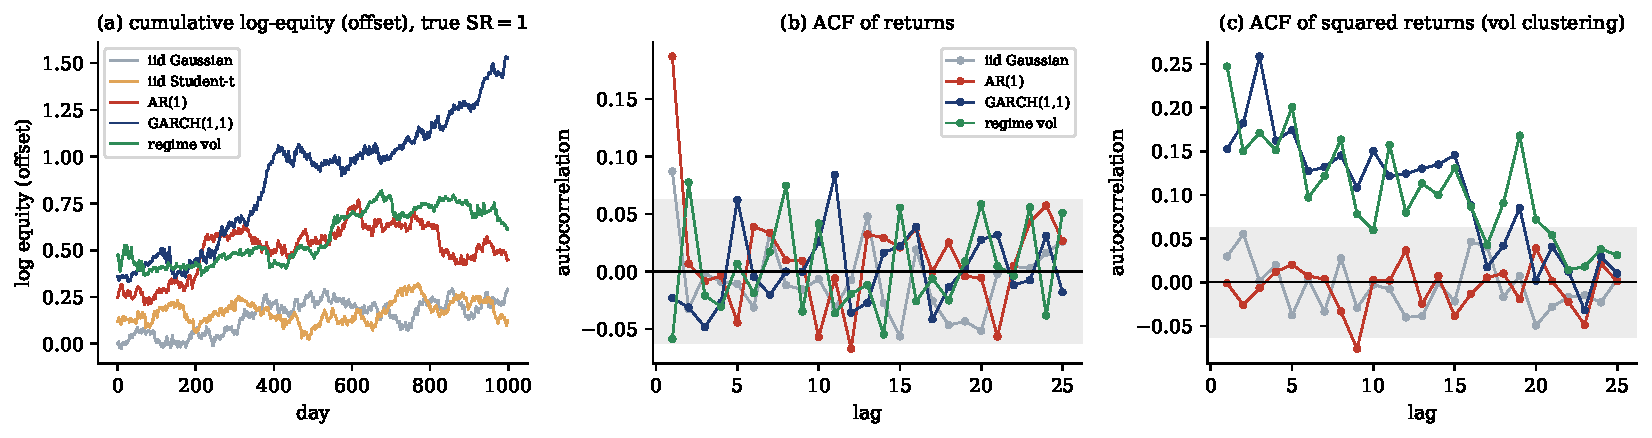
\includegraphics[width=\textwidth]{fig_setup.pdf}
\caption{The five DGP families at their canonical parameters (true
$\sr=1$, $\sigma=1\%$/day, $T=1000$). (a) Cumulative log-equity (vertically
offset for legibility). (b) Sample autocorrelation of returns: only the AR(1)
family (here $\phi=0.2$) is serially correlated in levels. (c) Sample
autocorrelation of squared returns: GARCH(1,1) and regime-switching volatility
cluster strongly, while their return levels remain uncorrelated. Panels (b)
and (c) show the four dependence-relevant families (iid Student-$t$, whose
ACFs match iid Gaussian, is omitted there for legibility). The shaded
band is the approximate $\pm 1.96/\sqrt{T}$ null range.}
\label{fig:setup}
\end{figure}

\paragraph{Sampled design.} Every experiment draws its own fully recorded
configuration: true annualized Sharpe uniform on $[0,2]$; daily volatility
uniform on $[0.005,0.02]$ (roughly $8$--$32\%$ annualized); the drift is then
set to $\mu = \sr\,\sigma/\sqrt{252}$ so the true Sharpe is exact by
construction. Family-specific parameters: $\nu\in\{5,6,8,12,20\}$;
$\phi\in\{0.05,0.10,0.20,0.30\}$; GARCH $\alpha$ uniform on $[0.03,0.12]$ with
persistence $\alpha+\beta$ uniform on $[0.85,0.98]$; regime volatility ratio
uniform on $[2,4]$ with stay probabilities uniform on $[0.95,0.99]$ (low state)
and $[0.90,0.98]$ (high state). There are no hidden per-draw constants: every
sampled parameter of every experiment is recorded in the released data, and the
sampling ranges themselves are recorded in the results metadata.

\section{Experimental setup}
\label{sec:setup}

\paragraph{Sharpe coverage.} We run $400$ experiments per (family, $T$) cell
over $T\in\{250,1000,4000\}$---$6{,}000$ experiments in all. Each experiment
generates one sample, builds all fourteen intervals at $90\%$ and $95\%$
nominal from that same sample ($B=2{,}000$), and records whether each interval
covers the known true Sharpe, plus its width. Coverage estimates carry Wilson
$95\%$ binomial intervals; with several hundred such intervals across the
coverage tables, a handful of borderline significance calls are expected by
multiplicity alone, so we lean on patterns across cells rather than single
bold entries. At $n=400$ per cell the Wilson half-width is about
$\pm 0.02$--$0.04$.

\paragraph{Maximum drawdown.} For each family we fix one canonical
mid-range configuration (true $\sr=1$, $\sigma=1\%$/day; $\nu=6$; $\phi=0.2$;
$\alpha=0.08,\beta=0.88$; volatility ratio $3$ with stay probabilities
$0.98/0.95$) and $T\in\{250,1000\}$. The \emph{true} sampling distribution of
the length-$T$ maximum drawdown is estimated once per configuration from
$20{,}000$ independent paths (seeded and cached). Each of $150$ experiments
per (family,~$T$) cell---$1{,}500$ in all---then draws one sample, lets every
eligible method predict the $q$-quantile $\hat q$ of the drawdown distribution,
and records the \emph{realized} tail probability
$F_{\text{true}}(\hat q) = \mathbb P_{\text{true}}(\mdd \le \hat q)$. For a
calibrated method the mean realized probability equals the nominal $q$.

\paragraph{Reproducibility.} Every experiment receives its own
\texttt{SeedSequence}-spawned generator in a fixed order, so all numbers are
bit-identical regardless of worker count. The full run takes about six minutes
on a laptop ($331$ s in the released results).

\section{Results}

\subsection{Where the advice holds: iid returns, heavy tails included}
\label{sec:iid}

Table~\ref{tab:iid} pools the $2{,}400$ experiments on the two iid families.
The practitioner recipe is calibrated where its assumption holds: at $95\%$
nominal the iid percentile bootstrap covers $0.954$ $[0.945,0.961]$, the basic
and BCa variants $0.952$, and Lo's iid standard error $0.953$. The trade-level
resamplers sit between $0.93$ and $0.95$: the $5$-day and threshold-crossing
(CUSUM) segmentations are calibrated ($0.948$ and $0.949$), while the $21$-day
segmentation undercovers mildly ($0.931$)---not because of dependence (there
is none) but because at $T=250$ it leaves only $\lfloor 250/21\rfloor = 11$
resampling units, too few for stable tail quantiles. The same
small-$T$ inefficiency, amplified, explains the fixed long-block stationary
bootstraps: $L=20$ covers $0.932$ and $L=50$ only $0.907$ at $95\%$ pooled.
The automatic-length block bootstraps are indistinguishable from the iid
bootstrap here ($0.953$, $0.950$)---on iid data the Politis--White rule
correctly collapses to a mean block length of about $1.0$--$1.1$ days, i.e.\
it recovers the iid bootstrap.

Heavy tails do not break the percentile bootstrap. On the Student-$t$ family
the percentile interval covers $0.945/0.938/0.970$ at $95\%$ across
$T=250/1000/4000$; restricting to the heaviest tail sampled ($\nu=5$, where
the fourth moment barely exists, $n=266$) gives $0.962$ at $95\%$ and $0.906$
at $90\%$. Lo's normal-theory standard error survives these tails as well at
the sample sizes studied. The failures documented below are therefore not
about tails; they are about dependence.

\begin{table}[t]
\centering
\caption{The honest positive: coverage on truly iid returns ($2{,}400$
experiments pooled over both iid families and all $T$). Brackets are Wilson
$95\%$ intervals on the coverage estimate; \textbf{bold} marks significant
undercoverage (Wilson interval entirely below nominal).}
\label{tab:iid}
\small
\begin{tabular}{lcc}
\toprule
Method & coverage at $90\%$ nominal & coverage at $95\%$ nominal \\
\midrule
Lo iid SE             & 0.902 [0.890, 0.914] & 0.953 [0.944, 0.961] \\
Lo HAC SE             & 0.897 [0.884, 0.908] & 0.949 [0.940, 0.957] \\
iid boot (percentile) & 0.902 [0.889, 0.913] & 0.954 [0.945, 0.961] \\
iid boot (basic)      & 0.903 [0.891, 0.915] & 0.952 [0.943, 0.960] \\
iid boot (BCa)        & 0.902 [0.890, 0.914] & 0.952 [0.942, 0.960] \\
trade resample (5d)   & 0.892 [0.879, 0.904] & 0.948 [0.938, 0.956] \\
trade resample (21d)  & \textbf{0.876} [0.862, 0.889] & \textbf{0.931} [0.920, 0.940] \\
trade resample (cusum)& 0.893 [0.880, 0.905] & 0.949 [0.939, 0.957] \\
stationary $L{=}5$    & 0.895 [0.882, 0.906] & 0.951 [0.941, 0.959] \\
stationary $L{=}10$   & \textbf{0.885} [0.872, 0.897] & 0.943 [0.932, 0.951] \\
stationary $L{=}20$   & \textbf{0.874} [0.860, 0.886] & \textbf{0.932} [0.922, 0.942] \\
stationary $L{=}50$   & \textbf{0.845} [0.830, 0.859] & \textbf{0.907} [0.895, 0.918] \\
stationary auto       & 0.901 [0.888, 0.912] & 0.953 [0.943, 0.960] \\
circular auto         & 0.900 [0.887, 0.911] & 0.950 [0.940, 0.958] \\
\bottomrule
\end{tabular}
\end{table}

\subsection{Autocorrelation breaks iid resampling---asymptotically}
\label{sec:ar}

Table~\ref{tab:dependent} is the headline: coverage at $95\%$ nominal on the
three dependent families, stratified by $T$ (the $90\%$ panorama over all
fifteen family$\times T$ cells is Figure~\ref{fig:heatmap}; the full table
with Wilson intervals and widths is in the released \texttt{results.json}).
Two of the three dependent families turn out to be nearly harmless for Sharpe
coverage. Under GARCH(1,1) and regime-switching volatility the iid percentile
bootstrap covers $0.885$--$0.915$ at $90\%$ nominal across all cells, and
binning the GARCH experiments by persistence shows only a mild slide, from
$0.907$ in the lowest-persistence quartile to $0.890$ in the highest (mean
$\alpha+\beta = 0.962$; Figure~\ref{fig:degradation}b). The reason is
structural: these processes leave the \emph{level} of returns serially
uncorrelated, and the sampling variance of the Sharpe estimator is driven by
the long-run covariance of $(r_t, r_t^2)$---volatility clustering enters only
through the second component, a second-order effect at these persistence
levels, sample sizes, and Sharpe levels (daily $\sr$ is at most $0.13$ in our
designs, which suppresses the $r_t^2$ channel's weight).

\begin{figure}[t]
\centering
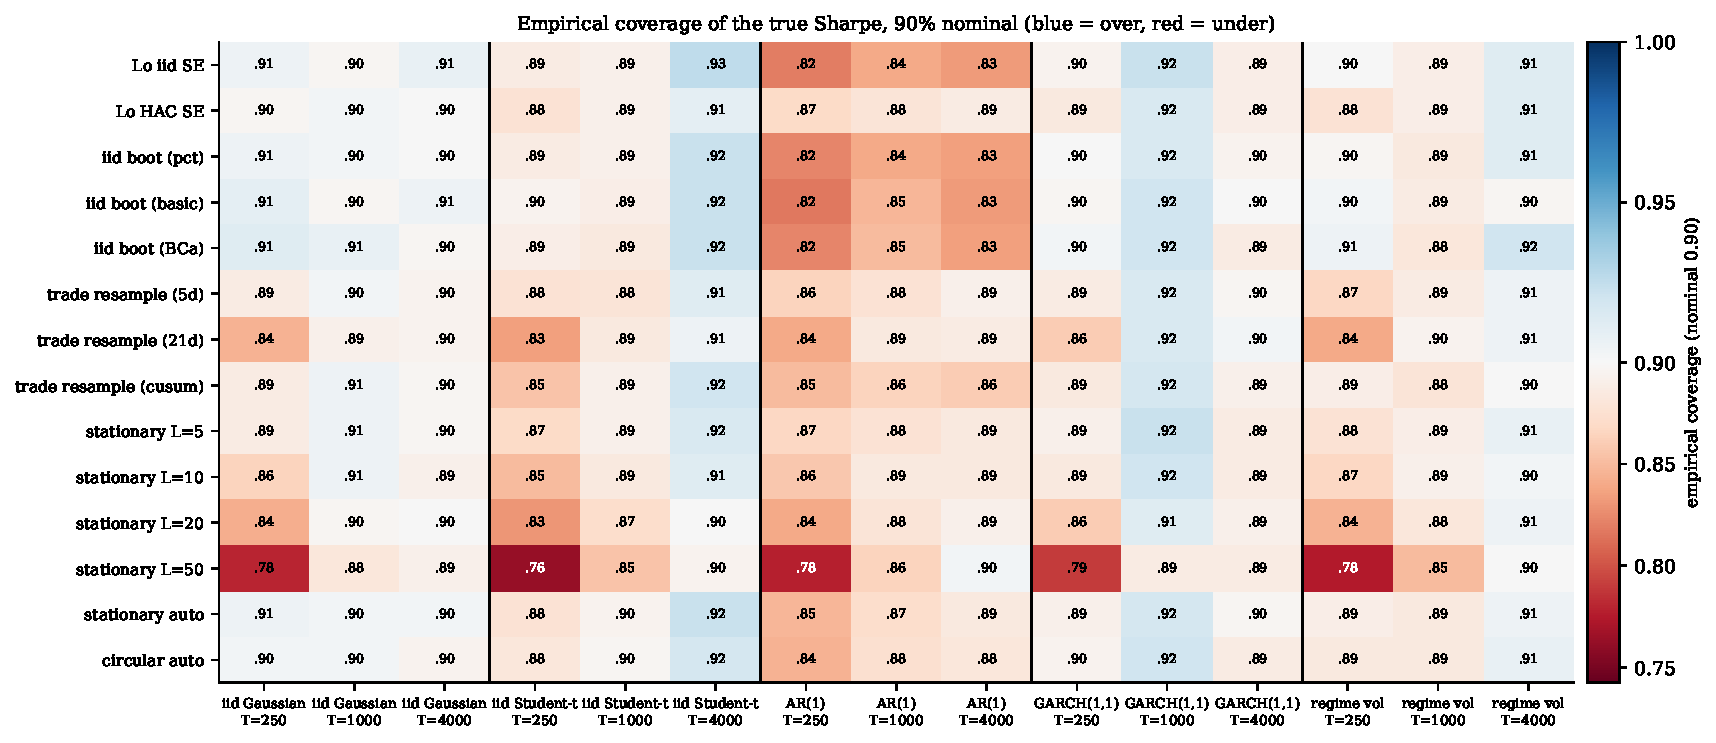
\includegraphics[width=\textwidth]{fig_coverage_heatmap.pdf}
\caption{Empirical coverage of the true Sharpe at $90\%$ nominal, all fourteen
methods (rows) by family and sample length (columns); $400$ experiments per
cell. Red marks undercoverage, blue overcoverage. The AR(1) columns are red for
every iid-resampling and analytic-iid method at every $T$; the long fixed
block ($L{=}50$) column at $T{=}250$ is the deepest red everywhere; GARCH and
regime columns are close to nominal throughout.}
\label{fig:heatmap}
\end{figure}

\begin{table}[t]
\centering
\caption{Headline coverage at $95\%$ nominal on the dependent DGPs, by family
and sample length ($400$ experiments per cell; Wilson half-widths
$\pm 0.018$--$0.035$). \textbf{Bold} marks significant undercoverage. The iid
families are in Table~\ref{tab:iid}; the $90\%$ level is shown in
Figure~\ref{fig:heatmap} and tabulated in \texttt{results.json}.}
\label{tab:dependent}
\small
\setlength{\tabcolsep}{4.5pt}
\begin{tabular}{lccc@{\hskip 1.4em}ccc@{\hskip 1.4em}ccc}
\toprule
& \multicolumn{3}{c}{AR(1)} & \multicolumn{3}{c}{GARCH(1,1)} & \multicolumn{3}{c}{regime vol}\\
\cmidrule(lr){2-4}\cmidrule(lr){5-7}\cmidrule(lr){8-10}
Method & 250 & 1000 & 4000 & 250 & 1000 & 4000 & 250 & 1000 & 4000 \\
\midrule
Lo iid SE             & \textbf{0.892} & \textbf{0.892} & \textbf{0.910} & 0.953 & 0.963 & 0.958 & 0.948 & 0.938 & 0.953 \\
Lo HAC SE             & 0.938 & \textbf{0.927} & 0.958 & 0.948 & 0.968 & 0.960 & 0.948 & 0.945 & 0.953 \\
iid boot (percentile) & \textbf{0.885} & \textbf{0.892} & \textbf{0.907} & 0.950 & 0.960 & 0.955 & 0.950 & 0.938 & 0.953 \\
iid boot (basic)      & \textbf{0.900} & \textbf{0.900} & \textbf{0.900} & 0.960 & 0.968 & 0.950 & 0.948 & 0.938 & 0.948 \\
iid boot (BCa)        & \textbf{0.887} & \textbf{0.890} & \textbf{0.907} & 0.953 & 0.968 & 0.958 & 0.948 & 0.940 & 0.950 \\
trade resample (5d)   & 0.943 & \textbf{0.925} & 0.955 & 0.943 & 0.963 & 0.960 & 0.935 & 0.935 & 0.948 \\
trade resample (21d)  & \textbf{0.895} & 0.935 & 0.953 & \textbf{0.915} & 0.960 & 0.953 & \textbf{0.895} & 0.938 & 0.943 \\
trade resample (cusum)& \textbf{0.895} & \textbf{0.907} & \textbf{0.925} & 0.943 & 0.965 & 0.955 & 0.943 & 0.938 & 0.950 \\
stationary $L{=}5$    & 0.935 & \textbf{0.925} & 0.950 & 0.940 & 0.968 & 0.963 & 0.938 & 0.935 & 0.953 \\
stationary $L{=}10$   & 0.930 & 0.930 & 0.953 & 0.932 & 0.963 & 0.958 & \textbf{0.925} & 0.935 & 0.948 \\
stationary $L{=}20$   & \textbf{0.907} & \textbf{0.922} & 0.955 & \textbf{0.912} & 0.953 & 0.953 & \textbf{0.897} & 0.935 & 0.940 \\
stationary $L{=}50$   & \textbf{0.845} & \textbf{0.910} & 0.955 & \textbf{0.863} & 0.940 & 0.943 & \textbf{0.868} & \textbf{0.912} & 0.940 \\
stationary auto       & \textbf{0.917} & \textbf{0.922} & 0.953 & 0.950 & 0.963 & 0.960 & 0.945 & 0.935 & 0.953 \\
circular auto         & \textbf{0.912} & \textbf{0.927} & 0.948 & 0.955 & 0.968 & 0.953 & 0.945 & 0.932 & 0.948 \\
\bottomrule
\end{tabular}
\end{table}

Autocorrelation is a different story. Figure~\ref{fig:degradation}a tracks
$90\%$-nominal coverage against the AR(1) coefficient (pooled over $T$,
roughly $300$ experiments per $\phi$ value): the iid percentile bootstrap
degrades from $0.915$ at $\phi=0.05$ to $0.811$, $0.834$, and $0.777$ at
$\phi=0.10$, $0.20$, $0.30$ (adjacent-$\phi$ differences are within Wilson
noise; it is the trend, not each step, that is monotone). Table~\ref{tab:phi03} zooms into the worst cell,
$\phi=0.3$ ($n=296$). At $95\%$ nominal the per-bar iid bootstrap covers
$0.841$ $[0.795,0.878]$: an interval sold as missing $5\%$ of the time misses
$15.9\%$ of the time, more than three times the nominal rate.

Two features make this failure structural rather than incidental. First,
\emph{it does not vanish with sample size}: at $95\%$ nominal the per-$T$
coverage at $\phi=0.3$ is $0.812$, $0.856$, $0.854$ for $T=250,1000,4000$ (at
$90\%$: $0.719$, $0.798$, $0.812$). The iid bootstrap converges---to an
interval calibrated for the wrong sampling variance. Under positive
autocorrelation the variance of $\widehat\sr$ is inflated by a factor that
survives $T\to\infty$, and intervals built from independently resampled bars
are too narrow by exactly that factor, at every sample size: the limiting
coverage of an iid-variance interval under AR(1) is
$2\Phi\!\big(z_{\alpha/2}\sqrt{(1-\phi)/(1+\phi)}\big)-1$, which at
$\phi=0.3$ equals $0.850$ at $95\%$ nominal and $0.773$ at $90\%$---our
$T=4000$ cells ($0.854$ and $0.812$) sit on that asymptote. (Per-$T$ cells
have $n\approx 96$--$104$, Wilson half-width ${\sim}0.07$, so the supported
per-$T$ statement is that $T=4000$ coverage still significantly excludes
nominal, not that adjacent $T$ cells differ.) Second, \emph{the
interval construction is irrelevant}: percentile $0.841$, basic $0.848$, BCa
$0.838$. The BCa machinery corrects bias and skewness of the bootstrap
distribution; it cannot correct a bootstrap distribution whose dispersion is
wrong. Lo's iid standard error fails identically ($0.841$)---it shares the
assumption, not the mechanism. What fixes the cell is modeling the dependence:
Lo's HAC variant covers $0.946$, the $5$-day trade resampler $0.946$, the
circular block bootstrap $0.946$, the automatic stationary bootstrap $0.939$.

\begin{figure}[t]
\centering
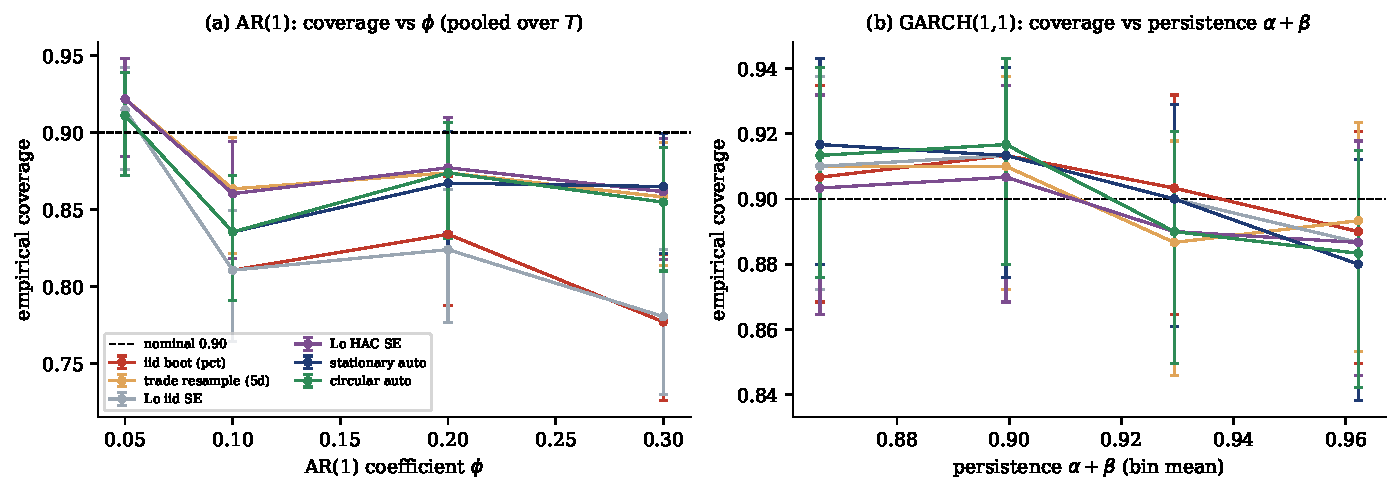
\includegraphics[width=\textwidth]{fig_degradation.pdf}
\caption{Coverage degradation with dependence strength at $90\%$ nominal
(pooled over $T$; error bars are Wilson $95\%$ intervals). (a) Against the
AR(1) coefficient $\phi$: the iid-assumption methods (iid percentile, Lo iid)
fall to $0.78$ at $\phi=0.3$ while the dependence-aware methods (Lo HAC,
trade-5d, stationary/circular auto) stay near $0.86$; none reaches nominal,
mostly due to the $T{=}250$ stratum. (b) Against GARCH persistence
$\alpha+\beta$ (quartile bins): all methods stay within a few points of
nominal, drifting slightly low only in the highest-persistence bin.}
\label{fig:degradation}
\end{figure}

\begin{table}[t]
\centering
\caption{The worst autocorrelation cell: AR(1) with $\phi=0.3$ ($n=296$
pooled; $96/104/96$ per $T$). Coverage at both nominal levels pooled over
$T$, then the $95\%$ level stratified by $T$: the iid-resampling failure does
not shrink as the sample grows. \textbf{Bold} marks significant
undercoverage.}
\label{tab:phi03}
\small
\begin{tabular}{lcc@{\hskip 1.8em}ccc}
\toprule
& \multicolumn{2}{c}{pooled over $T$} & \multicolumn{3}{c}{$95\%$ nominal, by $T$}\\
\cmidrule(lr){2-3}\cmidrule(lr){4-6}
Method & at $90\%$ & at $95\%$ & 250 & 1000 & 4000 \\
\midrule
Lo iid SE             & \textbf{0.780} & \textbf{0.841} & \textbf{0.812} & \textbf{0.856} & \textbf{0.854} \\
Lo HAC SE             & \textbf{0.861} & 0.946 & 0.917 & 0.952 & 0.969 \\
iid boot (percentile) & \textbf{0.777} & \textbf{0.841} & \textbf{0.812} & \textbf{0.856} & \textbf{0.854} \\
iid boot (basic)      & \textbf{0.780} & \textbf{0.848} & \textbf{0.823} & \textbf{0.865} & \textbf{0.854} \\
iid boot (BCa)        & \textbf{0.780} & \textbf{0.838} & \textbf{0.812} & \textbf{0.846} & \textbf{0.854} \\
trade resample (5d)   & \textbf{0.858} & 0.946 & 0.927 & 0.952 & 0.958 \\
trade resample (21d)  & \textbf{0.858} & 0.929 & \textbf{0.865} & 0.962 & 0.958 \\
trade resample (cusum)& \textbf{0.828} & \textbf{0.875} & \textbf{0.844} & \textbf{0.894} & \textbf{0.885} \\
stationary $L{=}5$    & \textbf{0.855} & 0.932 & \textbf{0.885} & 0.952 & 0.958 \\
stationary $L{=}10$   & 0.868 & 0.929 & \textbf{0.865} & 0.952 & 0.969 \\
stationary $L{=}20$   & 0.872 & 0.929 & \textbf{0.865} & 0.962 & 0.958 \\
stationary $L{=}50$   & \textbf{0.851} & \textbf{0.905} & \textbf{0.812} & 0.942 & 0.958 \\
stationary auto       & \textbf{0.865} & 0.939 & \textbf{0.885} & 0.962 & 0.969 \\
circular auto         & \textbf{0.855} & 0.946 & \textbf{0.906} & 0.962 & 0.969 \\
\bottomrule
\end{tabular}
\end{table}

\subsection{The trade-resampling nuance: an accidental block bootstrap}
\label{sec:trade}

The practitioner recipe's preferred unit is the \emph{trade}, not the bar, and
this turns out to matter enormously---in the recipe's favor. Resampling
fixed-length $5$-day episodes is algebraically a non-overlapping block
bootstrap with block length $5$, and five days comfortably exceeds the
dependence length of an AR(1) with $\phi\le0.3$ (autocorrelation
$0.3^5\approx0.002$ five bars out). Accordingly, at $\phi=0.3$ and $95\%$
nominal the $5$-day trade resampler covers $0.946$ $[0.914,0.966]$ where the
per-bar iid bootstrap covers $0.841$ $[0.795,0.878]$
(Table~\ref{tab:phi03})---fully calibrated, by accident of unit choice rather
than by design.

The conditions for the accident to work are visible in the same tables.
\emph{The unit must exceed the dependence length}: the threshold-crossing
(CUSUM) segmentation produces episodes averaging about $6$ days on the AR(1)
family ($5.6$ at $\phi=0.3$), but their lengths are variable and
data-dependent---fast threshold crossings produce many short episodes---and
its coverage lands in between, $0.875$ at $\phi=0.3$ ($95\%$), significantly
under nominal. \emph{And the number of units must stay large}: the $21$-day
segmentation handles the dependence ($0.962$ at $\phi=0.3$, $T=1000$) but
undercovers at $T=250$ ($0.865$) for the same reason it undercovers on iid
data there---eleven resampling units cannot pin a $95\%$ quantile. The per-bar
version of the recipe is simply the degenerate case: a ``trade'' of one bar,
which is the failure mode of Section~\ref{sec:ar}.

This reframes the practitioner advice rather than vindicating or damning it:
``resample trades'' is sound \emph{when trades are multi-day episodes}, because
it is then an unwitting block bootstrap whose block structure happens to match
the dependence; it is unsound when the resampling unit is a bar, a one-day
trade, or an episode distribution with many short members.

\subsection{Block length: the sweep, the automatic rule, and what width buys}
\label{sec:block}

The fixed-length sweep quantifies the block-length dilemma. Long blocks pay a
small-sample price: at $T=250$ and $90\%$ nominal, $L=50$ covers
$0.781$ pooled over the dependent families ($0.762$--$0.790$ per family,
including the iid ones)---with only five distinct blocks per resample, the
bootstrap distribution is too coarse and too narrow. Yet long blocks are
exactly what large-$T$ dependence wants: at $T=4000$ on AR(1), $L=50$ is the
\emph{best} method in the column ($0.902$ at $90\%$). No fixed $L$ wins
everywhere.

The automatic Politis--White rule navigates this trade-off about as well as a
data-driven rule can, and is one of the two methods we would recommend as a
default, but it is not magic. On iid families it correctly collapses to
$L\approx 1$ and reproduces the iid bootstrap. On AR(1) it chooses mean
lengths that grow with $T$ and $\phi$ ($\approx 3.8/6.1/10.9$ days at
$\phi=0.3$ for $T=250/1000/4000$) yet still undercovers, by $3.2$ points at
$90\%$ nominal pooled over the AR(1) family ($0.868$) and $1.9$ points at
$95\%$ ($0.931$). Part of this is the generic small-$T$ difficulty (below),
and part is that the rule optimizes the block length for the long-run variance
of the sample \emph{mean}, not for quantiles of a studentized ratio statistic
\citep{hall1995blocking,politis2004automatic}; its chosen lengths are, for
this purpose, slightly short.

Two cross-method facts deserve emphasis. First, \emph{at $T=250$ on the
dependent families, no method reaches nominal $90\%$ coverage}: the best of
the fourteen achieves $0.879$, and every Wilson interval excludes $0.90$. At
$95\%$ nominal only Lo's HAC standard error ($0.944$) and the $5$-day trade
resampler ($0.940$) are not significantly under. One year of daily data is
simply not enough for honest dependence-aware interval estimation at
conventional levels, by any of these methods. Second, the width--coverage
trade-off (Figure~\ref{fig:width}) shows there is no free narrowness: at
$T=250$ the methods that approach nominal coverage do so with intervals about
$4.1$ annualized-Sharpe units wide ($\pm 2$ around the estimate)---an honest
statement of how little one year of daily data constrains a Sharpe
ratio---while the narrow intervals ($L=50$ at width $3.4$) buy their width by
not covering. Pooling can also flatter a method: at $T=4000$ the BCa interval
is not significantly under nominal \emph{pooled} across the dependent families
($0.938$), yet its AR(1) stratum sits at $0.907$
(Table~\ref{tab:dependent})---averaging the harmless GARCH and regime columns
into the harmful AR(1) one hides the failure that matters. Coverage claims
should be read stratified.

\begin{figure}[t]
\centering
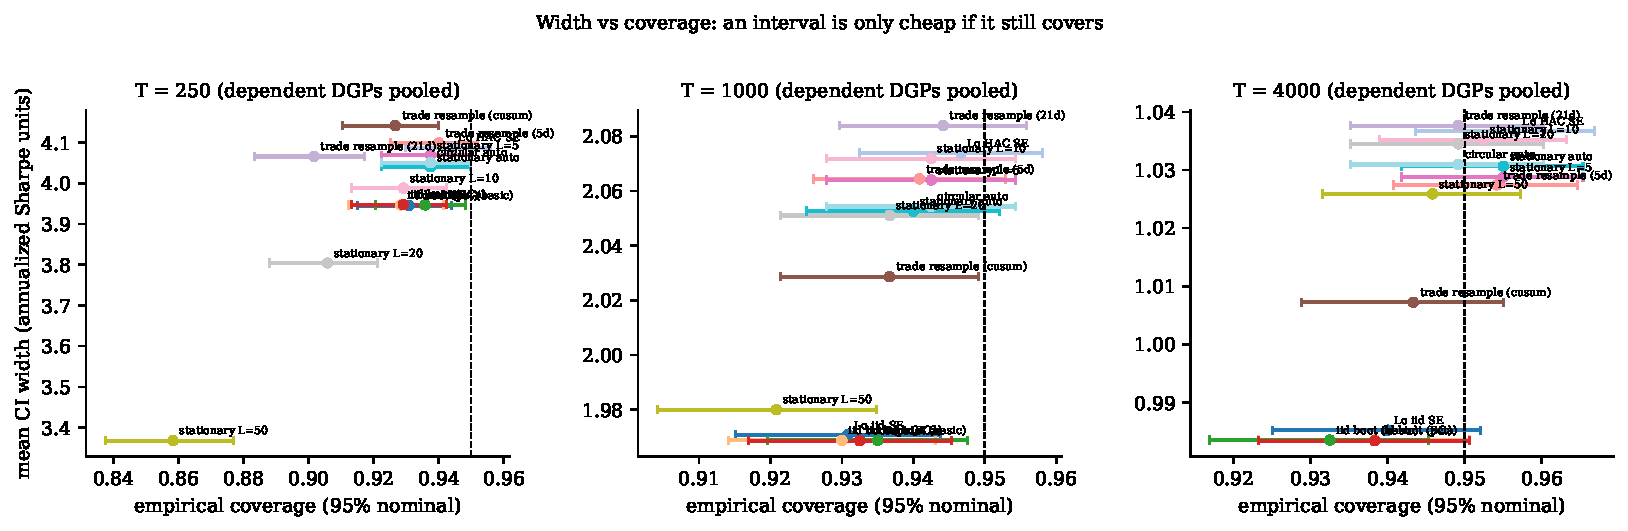
\includegraphics[width=\textwidth]{fig_width_coverage.pdf}
\caption{Mean interval width versus empirical coverage at $95\%$ nominal,
dependent DGPs pooled, one panel per $T$ (error bars: Wilson $95\%$ intervals;
dashed line: nominal). An interval is only cheap if it still covers: the
narrow iid-bootstrap and Lo-iid intervals sit left of nominal at every $T$,
the $L{=}50$ stationary bootstrap is narrowest and worst at $T{=}250$, and
the methods nearest nominal (Lo HAC, trade-5d, stationary/circular auto) pay
for coverage with the widest intervals.}
\label{fig:width}
\end{figure}

\subsection{Maximum drawdown: optimistic everywhere}
\label{sec:mdd}

The drawdown study asks each bootstrap to predict the $5\%$ worst-case
quantile of the maximum-drawdown distribution---the number a practitioner
quotes as ``with $95\%$ probability the drawdown will not be deeper than
this''---and scores the realized exceedance probability against the $20{,}000$-path
truth. Table~\ref{tab:mdd} reports the result: \emph{every} method is
optimistic on \emph{every} DGP. Even on iid Gaussian returns, where the
resampling scheme is correct, the realized exceedance of the iid bootstrap's
$q_{0.05}$ prediction is $0.102$ at $T=250$ and $0.082$ at $T=1000$---roughly
double nominal. The bootstrap sees only one realized path; its resamples
cannot produce drawdowns much deeper than the volatility and luck of that one
path allow, so the predicted tail quantile inherits estimation noise
asymmetrically. This is a plug-in bias, not a dependence effect, and it decays
only slowly with $T$.

Dependence then stacks on top. Under AR(1) the per-bar iid bootstrap's
exceedance is $0.232$ at $T=250$ and $0.226$ at $T=1000$---the ``$5\%$''
drawdown is a one-in-four event, and the bias does \emph{not} shrink with the
path length, for the same structural reason as in Section~\ref{sec:ar}.
Block methods repair most of this channel: at $T=1000$ the automatic
stationary bootstrap brings the AR(1) exceedance from $0.226$ down to
$0.115$, the $5$-day trade resampler to $0.112$ (at $T=250$ they reach only
$0.196$ and $0.143$). But under regime-switching volatility---returns
uncorrelated, variance persistent---block resampling fixes essentially
nothing: $0.165\to0.168$ at $T=250$, $0.134\to0.133$ at $T=1000$. The blocks
are far shorter than the regimes, so no resampling scheme in our set
reproduces the possibility that the \emph{next} path spends most of its life
in the high-volatility state. GARCH sits in between ($0.115/0.106$ iid
bootstrap, unimproved by blocks). Note the contrast with
Section~\ref{sec:ar}: volatility dynamics that barely move Sharpe
\emph{coverage} substantially poison drawdown \emph{tails}---the drawdown is
an extreme path functional and feels the clustering that the Sharpe
estimator's CLT averages out.

Even the predicted \emph{median} drawdown is biased under autocorrelation: the
per-bar bootstrap's $q_{0.50}$ is exceeded with probability $0.661$ ($T=250$)
and $0.696$ ($T=1000$) on AR(1), versus $0.51$--$0.61$ for the block methods.
In relative terms the per-bar $q_{0.05}$ prediction is about $15$--$17\%$ too
shallow on AR(1). Across our grid the realized probability of the nominal
$5\%$ drawdown ranges from $0.07$ to $0.23$: a practitioner quoting a
bootstrap ``$5\%$ worst-case drawdown'' should expect the true exceedance
probability to be $1.5$--$5$ times larger.

\begin{table}[t]
\centering
\caption{Maximum drawdown: mean realized exceedance probability
$F_{\text{true}}(\hat q_{0.05})$ of each method's nominal $5\%$ worst-case
quantile ($150$ experiments per cell; truth from $20{,}000$ paths per
configuration; canonical configs with true $\sr=1$). Calibrated $=0.05$;
larger means the predicted worst case is too shallow (optimistic). All cells
sit above nominal.}
\label{tab:mdd}
\small
\begin{tabular}{llccccc}
\toprule
Family & $T$ & iid pct & trade-5d & SB $L{=}20$ & SB auto & CB auto \\
\midrule
iid Gaussian & 250  & 0.102 & 0.111 & 0.161 & 0.102 & 0.102 \\
             & 1000 & 0.082 & 0.088 & 0.108 & 0.082 & 0.083 \\
iid Student-$t$ & 250  & 0.093 & 0.118 & 0.163 & 0.093 & 0.094 \\
             & 1000 & 0.074 & 0.077 & 0.094 & 0.074 & 0.074 \\
AR(1)        & 250  & 0.232 & 0.143 & 0.182 & 0.196 & 0.193 \\
             & 1000 & 0.226 & 0.112 & 0.121 & 0.115 & 0.111 \\
GARCH(1,1)   & 250  & 0.115 & 0.138 & 0.176 & 0.118 & 0.115 \\
             & 1000 & 0.106 & 0.110 & 0.138 & 0.105 & 0.105 \\
regime vol   & 250  & 0.165 & 0.181 & 0.227 & 0.168 & 0.169 \\
             & 1000 & 0.134 & 0.133 & 0.162 & 0.133 & 0.133 \\
\bottomrule
\end{tabular}
\end{table}

\section{Discussion}

The practitioner advice should be split into verdicts by regime and by
statistic, and each verdict is quantitative.

For the \emph{Sharpe ratio on genuinely iid PnL}, the advice is simply
correct: every variant---per-bar percentile bootstrap, trade resampling,
Lo's closed form---is calibrated, heavy tails included
(Table~\ref{tab:iid}). Nothing in our results justifies abandoning the iid
bootstrap where independence is credible.

For the \emph{Sharpe ratio under autocorrelated PnL}---overlapping positions,
slow signals, smoothed marks---per-bar iid resampling should never be used.
Its failure is not a finite-sample blemish that more data cures: at
$\phi=0.3$ the $95\%$ interval misses $15$--$19\%$ of the time at every
sample length up to $T=4000$, and upgrading the interval construction to BCa
changes nothing because the resampling scheme, not the quantile formula, is
wrong. The fix costs one line of code: a stationary or circular block
bootstrap with the corrected Politis--White automatic length, or Lo's HAC
standard error. Both are nearly calibrated everywhere here, with two honest
caveats: expect roughly $2$--$3$ points of residual undercoverage on
autocorrelated data at $T\le1000$, and expect \emph{no} method to deliver
nominal $90\%$ coverage at $T=250$ on dependent data---at that length the
honest interval is about $\pm2$ annualized Sharpe units wide, which is itself
the finding.

For \emph{trade-level resampling}, the verdict depends on the unit. Resampling
whole multi-day trades is an accidental non-overlapping block bootstrap and
inherits its calibration when the typical trade is longer than the dependence
length and the trade count is large ($0.946$ at $\phi=0.3$ for $5$-day
episodes); it degrades when episode lengths are variable with many short
members (CUSUM, $0.875$) and collapses to the per-bar failure as trades
approach one bar. A practitioner who wants to keep the trade-resampling
workflow should check the trade-length distribution against the PnL
autocorrelation length, and prefer the automatic block bootstrap when in
doubt---it needs no such check.

For \emph{maximum drawdown}, bootstrap quantiles should be treated as
optimistic lower bounds on the severity of the tail, under every method
tested. Block schemes remove the autocorrelation-driven part of the bias but
none of the volatility-regime part, and even the iid-on-iid case runs at twice
the nominal exceedance. A reported ``$5\%$ worst-case drawdown'' from $250$--$1000$
days of data behaved, in our grid, like a $7$--$23\%$ event; multiplying the
nominal tail probability by a factor of $1.5$ to $5$, or validating the
quantile against a parametric vol-clustering model, is the prudent reading.

\section{Limitations}

Our DGPs are stylized in disclosed ways. Innovations are Gaussian in the
dependent families, so heavy tails and dependence are never combined (the
Student-$t$ family is iid); AR(1) dependence is capped at $\phi=0.3$, and
real overlapping-position PnL can be more persistent; the regime and GARCH
parameter ranges, while drawn to be realistic, are choices. The trade-level
method is scored under a charitable reading---we resample trade episodes but
recompute the daily-frequency Sharpe, isolating the resampling question from
the per-trade units error in the circulated recipe; the fixed segmentation
drops a sub-window remainder, and the CUSUM threshold uses the full-sample
standard deviation, as a practitioner would compute it. We evaluate percentile
intervals for the block bootstraps as practitioners use them; studentized
block intervals with higher-order refinements \citep{ledoit2008robust} could
narrow the residual small-$T$ gap and are not tested. The Politis--White rule
is applied as published (it optimizes the sample-mean long-run variance, not
ratio-statistic quantiles). The drawdown truth is itself a $20{,}000$-path
Monte Carlo estimate (its quantile error is negligible relative to the
reported effects, though it is shared within a cell and so does not average
out across experiments), computed at one canonical parameter point per family
and $T\in\{250,1000\}$ only. Finally, true Sharpe ratios are sampled from
$[0,2]$ and all streams are univariate daily PnL: selection across many
backtests \citep{white2000reality,bailey2014deflated}, transaction costs, and
multi-asset effects are out of scope.

\section{Conclusion}

We gave the ``bootstrap your backtest'' advice its first controlled coverage
test, across fourteen interval methods, five data-generating processes with
exactly known annualized Sharpe ratios, and three sample lengths. The verdict
splits cleanly. On iid returns the advice is calibrated, heavy tails included:
the pooled $95\%$ percentile-bootstrap coverage is $0.954$. Under
autocorrelation the per-bar version is broken asymptotically, not just in
small samples---$0.841$ coverage at $95\%$ nominal for $\phi=0.3$, unimproved
from $T=250$ to $T=4000$ and unrescued by BCa---because the iid resampling
scheme converges to the wrong sampling variance. Resampling multi-day trades
is an accidental non-overlapping block bootstrap and is calibrated whenever
the trade unit exceeds the dependence length and trades are plentiful, which
is the regime in which the practitioner recipe quietly works. Automatic-length
block bootstraps and Lo's HAC standard error are the best general-purpose
defaults, within $2$--$3$ points of nominal everywhere except $T=250$, where
no method reaches nominal on dependent data. And for maximum drawdown every
bootstrap tested is optimistic on every process: the nominal $5\%$ worst-case
drawdown realized with probability $0.07$--$0.23$, with block methods fixing
only the autocorrelation channel. Resample blocks, not bars; report stratified
coverage, not pooled comfort; and read bootstrap drawdown quantiles as lower
bounds.

\paragraph{Reproducibility.} All experiments are deterministic given the
released seeds, and the worker count changes wall time only, never numbers. A
single command (\texttt{python scripts/run\_all.py}) regenerates every number
in about six minutes on a laptop, the package's \texttt{figures} module
regenerates every figure, and the script \texttt{check\_paper\_numbers.py}
asserts that every value quoted in this paper's tables and text matches the
generated results. The DGPs, interval
constructors, drawdown truth cache, and analysis are released as an
open-source package with tests.

\small
\bibliographystyle{plainnat}
\bibliography{refs}

\end{document}
